\chapter{G. Good Reports}

The following is a excerpt of places that people felt ``good''.

\begin{figure}[!htb]
  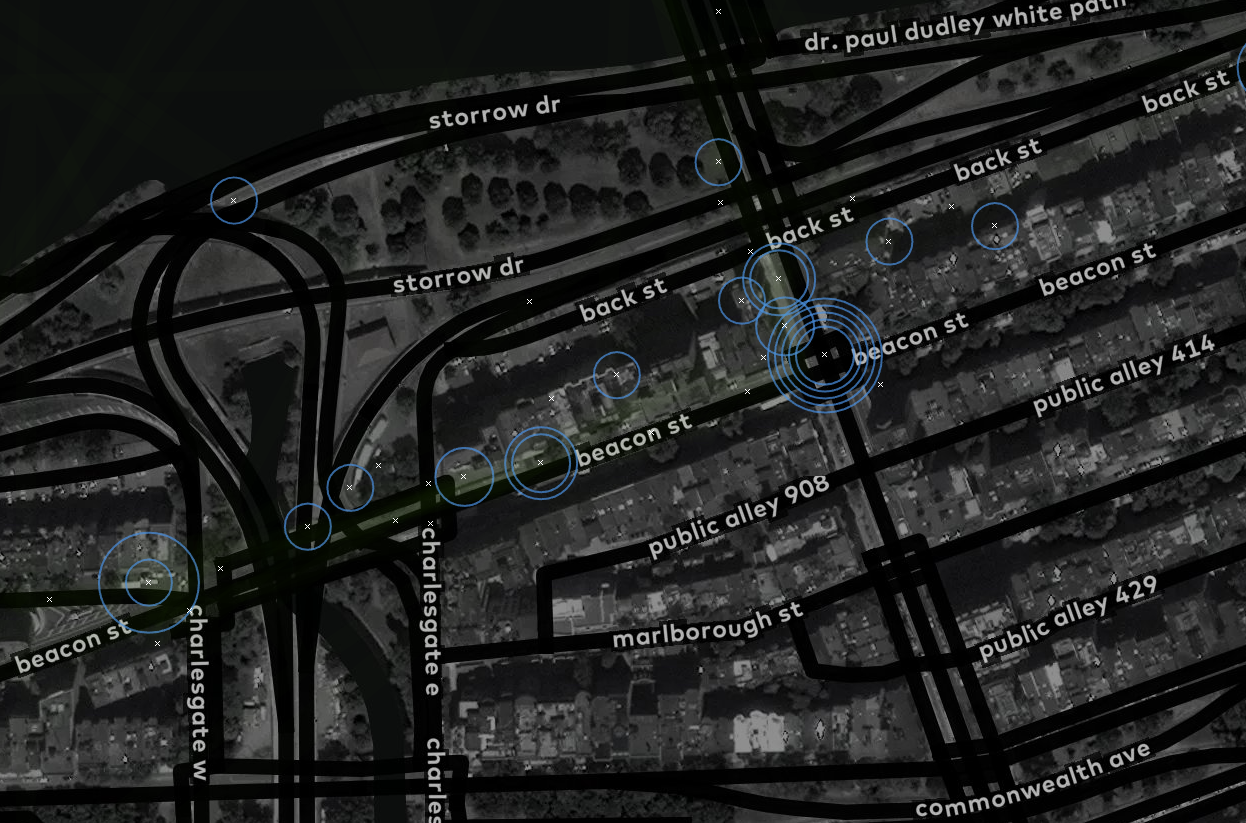
\includegraphics{appendix/G/fig/good_beacon.png}               
  \caption[``good'' reports in Massachusetts avenue and Beacon Street]{This result shows that the intervention had some successful outcomes in terms of perception. This place was marked as most dangerous in local media and the city has modified the path to be a protected bike lane. \nameref{appb:bad}}
  \label{fig:good_beacon}
\end{figure}

\begin{figure}[!htb]
  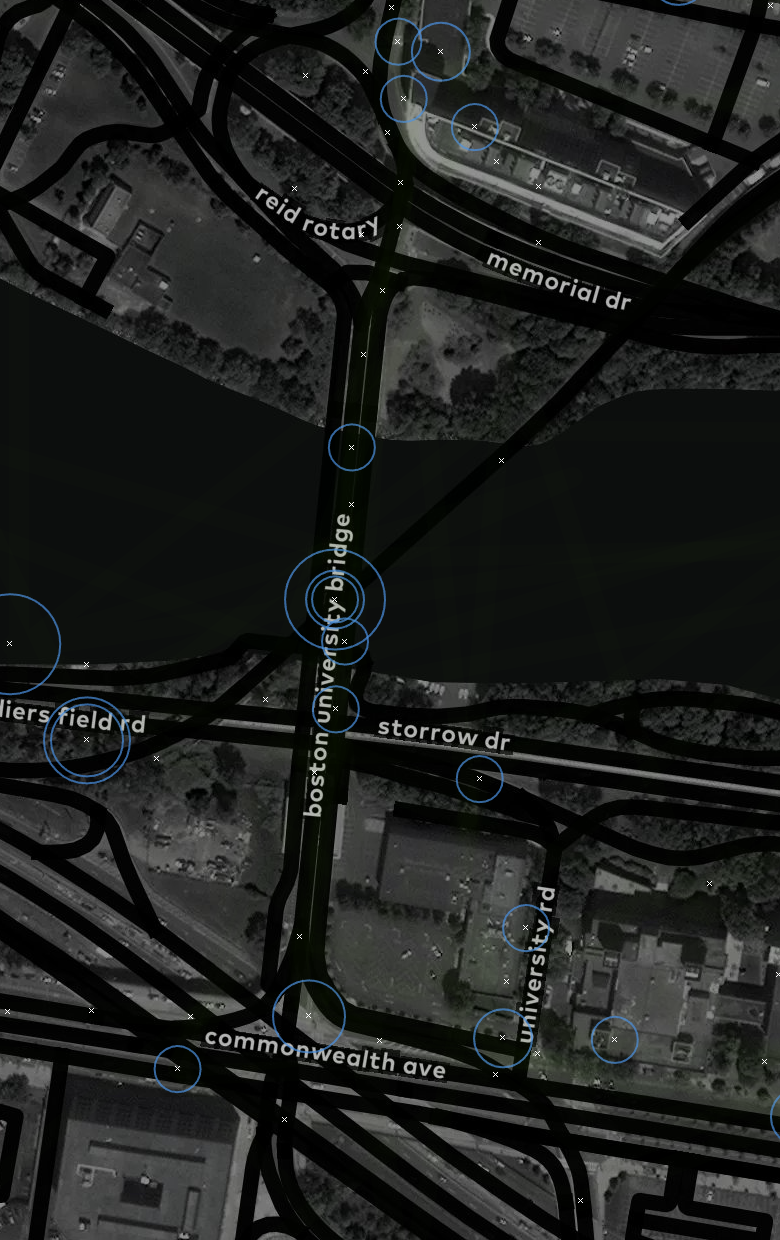
\includegraphics{appendix/G/fig/good_bu.png}               
  \caption[``good'' reports in BU bridge]{The BU bridge collected ``good'' reports in the middle, which may be a indicator that people felt good about the open scene. Users reported that the brdige was easy to pass and had good scenery.}
  \label{fig:good_bu}
\end{figure}

\begin{figure}[!htb]
  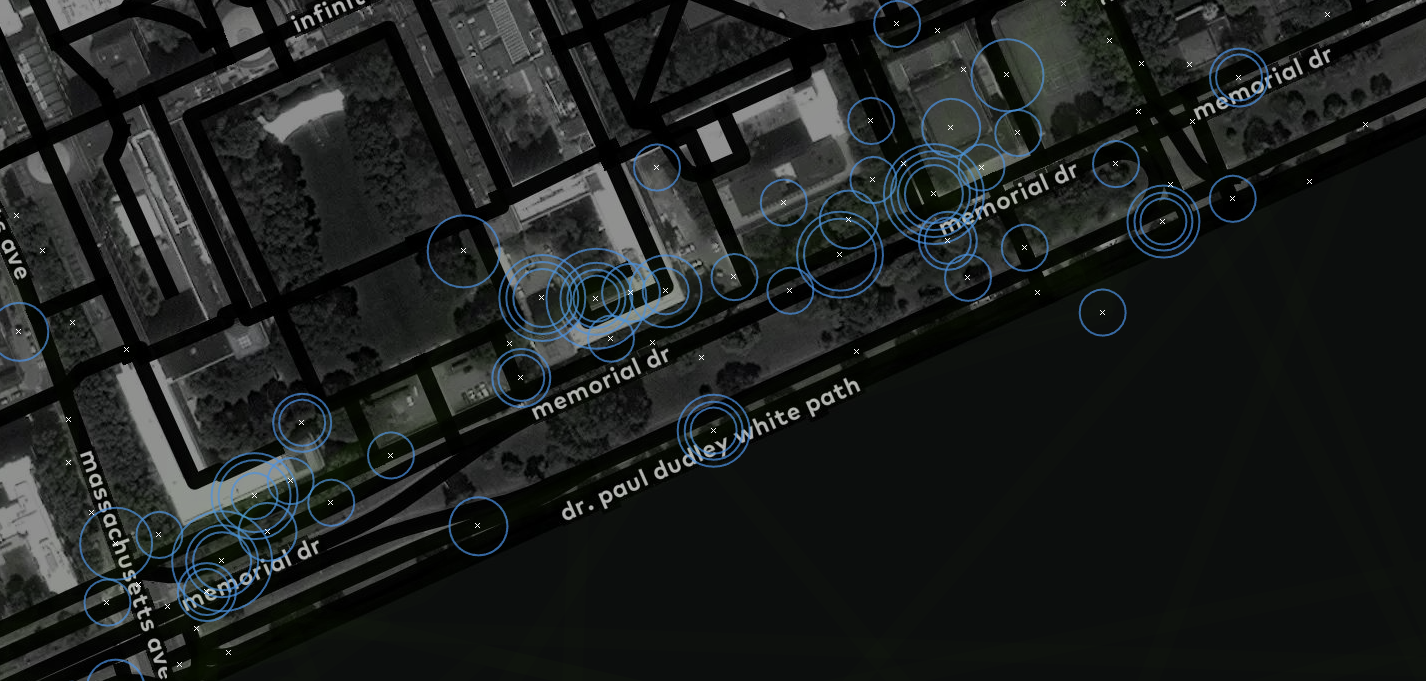
\includegraphics{appendix/G/fig/good_memorial.png}               
  \caption[``good'' reports in sidewalks of memorial drive]{Cambridge permits bikes to use the sidewalk of memorial drive, this path collected multiple ``good'' dings, despite where it is usually mixed traffic with pedestrians and potential for collisions.}
  \label{fig:good_memorial}
\end{figure}

\begin{figure}[!htb]
  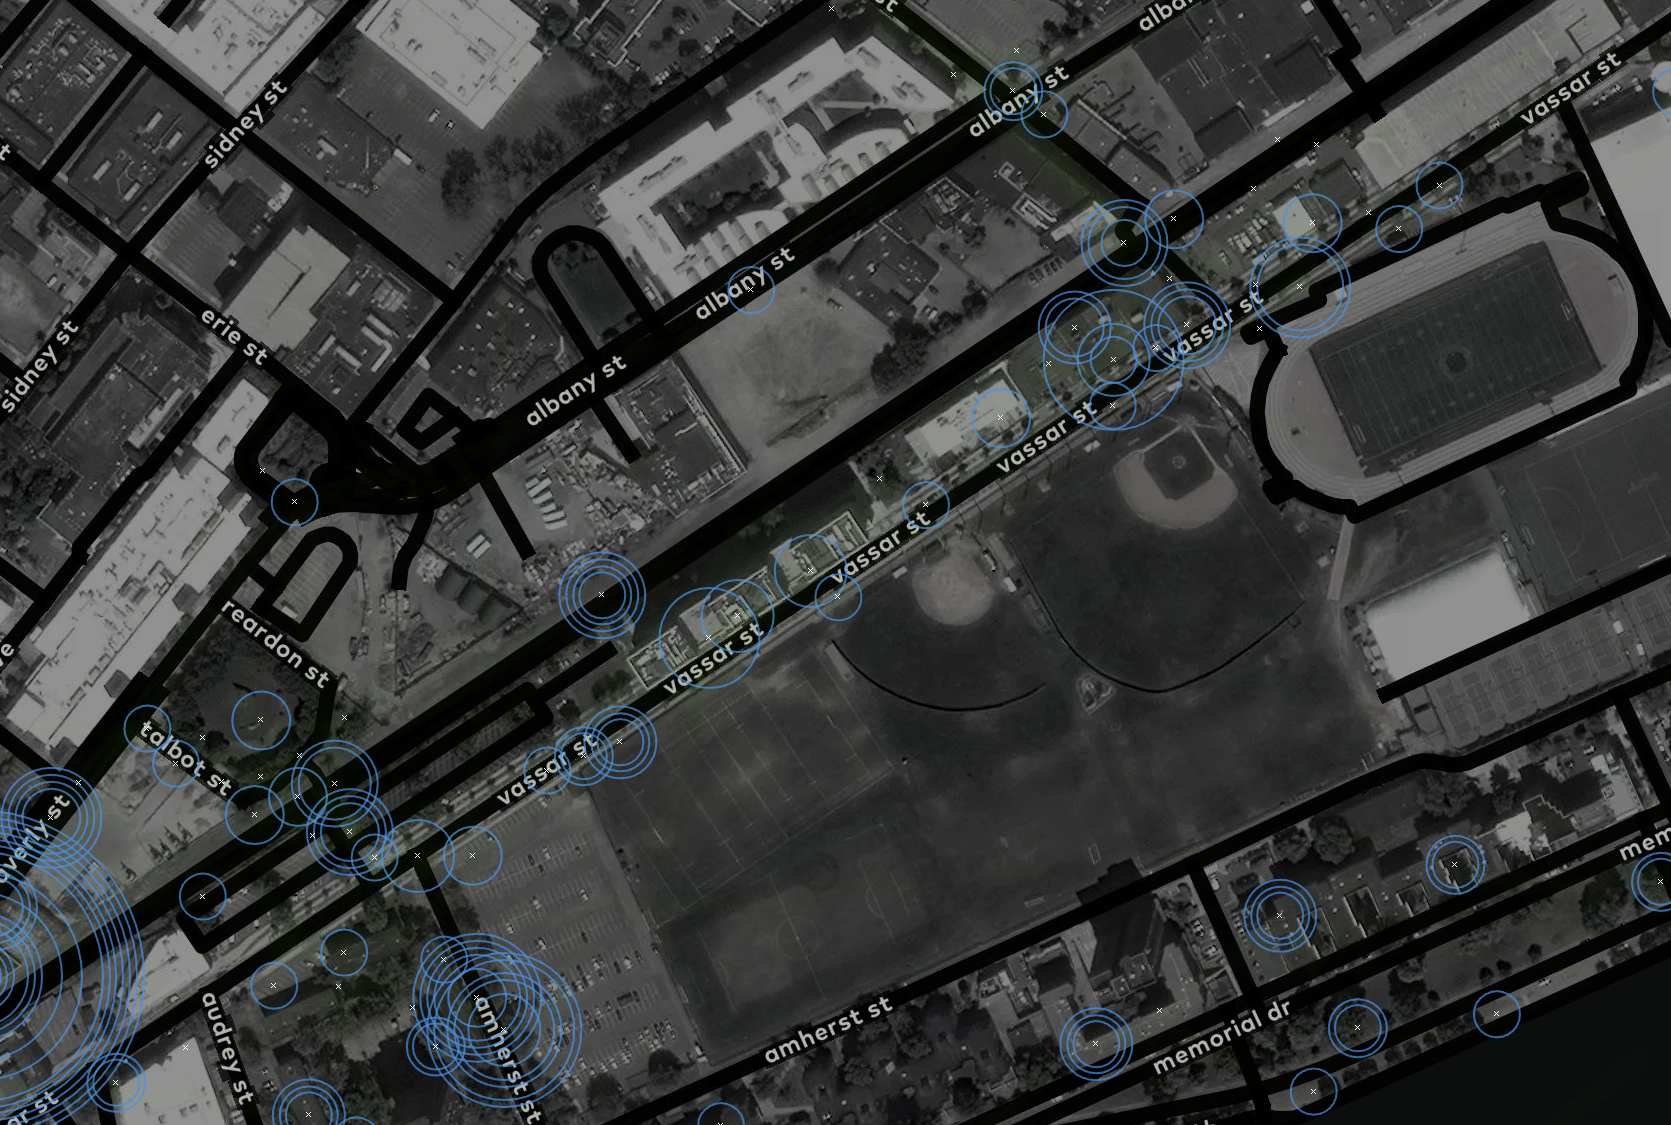
\includegraphics{appendix/G/fig/good_vassar.png}               
  \caption[``good'' reports in sidewalks of Vassar Street]{
  The path that collected the most ``good'' dings is Vassar Street, where the bike lane is separated with the car lane, at the same level of the side walk. The result shows that there is general tendency that roads with good infrastructure often had more good reports.}
  \label{fig:good_vassar}
\end{figure}